%
% File: chap03.tex
% Author: Antigoni Kourou
% Description: Methodology used for the research.
%
\let\textcircled=\pgftextcircled
\chapter{Methodology}
\label{chap:methods}
\initial{T}he proposed approach for an ontology-based feature extraction and opinion mining is composed by two important parts: pipeline coding and data analysis. For the first part, the code is written in Python 2.7. In addition to basic packages, I have made use of NLTK 3.2.1, py2neo 2.0.8, vaderSentiment, langdetect 1.0.1, WordNet 3.0 etc. All the codes belonging to the three first phases of the pipeline, excluding data analysis and visualization which will be treated later, can be found in Appendix II. 
\section{Dataset}
%
% HOW IS ARE THE REVIEWS RETRIEVED FROM AIRBNB
% FORMAT, CODE, TIME ...
%

Data from Airbnb listings in the Netherlands and UK has been collected over the past year by HAL24K\footnote{http://hal24k.com/}. Over a number of months in 2015 HAL24K recorded the active listings within the Netherlands and the UK and the associated accommodation descriptions and aggregate review scores of these listings. In March/April 2016 HAL24K revisited this known set of Airbnb listings and, for those that were still active, downloaded all of the text reviews that had been written by Airbnb users that had stayed at each listing up until the time of access. Approximately 1.5 million reviews were downloaded by HAL24K and stored within a Neo4j graph database maintaining the relationships between who had written the reviews, the reviews themselves and the accommodation about which the reviews were written. This corpus is filtered to be focused only in the data of Amsterdam for simplicity purposes and reduces the number of reviews in 71.2K, consisting in 2 356 listing which each listing has on average 30.2 reviews. The same pipeline can run in the bigger corpus, with the help of a more powerful machine. 
%
%

\section{Accommodation ontology} 
In knowledge management and Semantic Web research areas, ontologies are considered essential in order to describe various concepts and relationships between them. For the accommodation domain and related domains a few ontologies have been proposed, which cover different aspects in this domain. However these ontologies are often found as sub-ontologies of the e-tourism domain. In this research, the ontology of accommodation, shown in Figure \ref{fig:onto}, is based on several sources. Firstly HONTOLOGY \cite{chaves2012hontology}, which is brought in alignment with Accommodation in QALL-ME, Tourist Accommodationsin DBpedia.org and Lodging Business  in Schema.org, was initially created by following different scenarios of booking an accommodation and processing reviews in Web services. Secondly ACCO Accommodation Ontology \cite{hepp2013accommodation}, which is an extension of GoodRelations ontology \cite{hepp2008goodrelations}, is based on Owl Ontology Language (OWL) and is supported by Google and Yahoo for the e-commerce accommodation offers.
Besides these ontologies, features mentioned in the Web based accommodation services of AirBnb.com, Booking.com and TripAdvisor.com are covered. However, this paper extracts features for only a few part of the ontology, explicitly six features of Airbnb system: \textit{accuracy, check-in, cleanliness, communication, location} and \textit{value}.
For building a list of synonyms, hyponyms and hypernyms for these terms of ontology in order to increase the range of matches found in the text, the pipeline uses human-interaction. Thus, for every term the suitable definition to accommodation field is chosen manually in this case. The lists of related term is based on the Synsets and relations between concepts as introduced by WordNet 3.0 library and which is read by Python 2.7. They can be found in Appendix III.
\begin{figure}[h!]
	\centering
	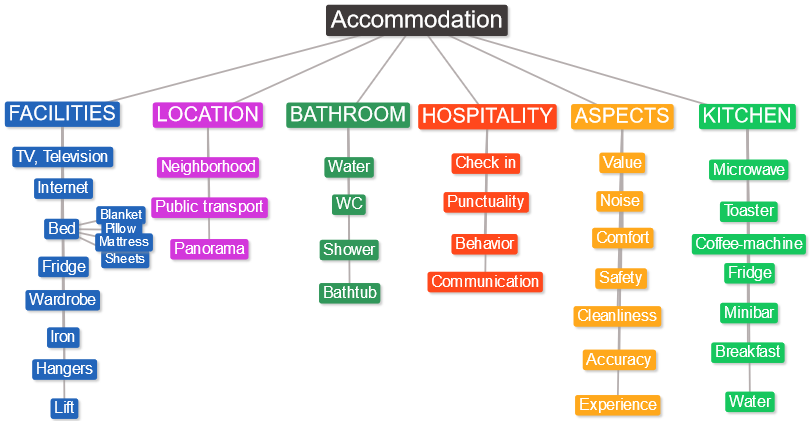
\includegraphics[height=0.3\textheight]{Ontology_of_accommodation}
	\caption{Example of the accommodation ontology}
	\label{fig:onto}
\end{figure}